%%%%%%%%%%%%%%%%%%%%%%%%%%%%%%%%
\subsection{Objetivo}
% ----------------------------------------------------------------------------
\begin{frame}{Reconhecimento de Voz}

\begin{figure}
	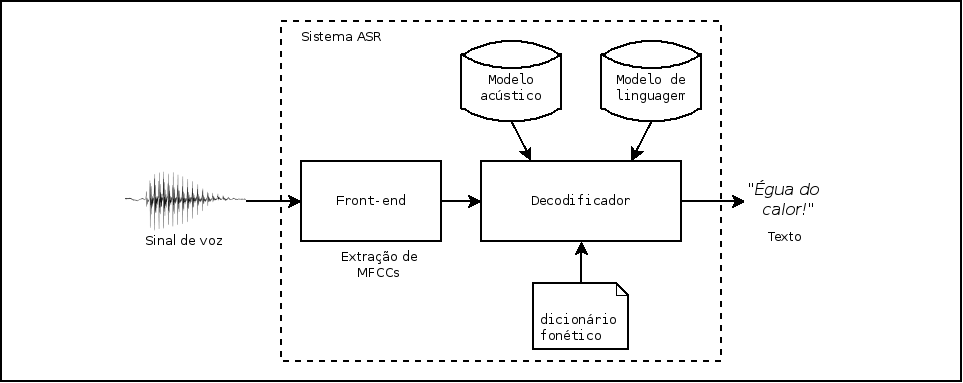
\includegraphics[width=0.4\textwidth]{Figures/asr}
    \caption{Esquema tradicional de um sistema autom\'atico de reconhecimento de voz}
\end{figure}

\begin{itemize}
    \item Aplica\c c\~oes:
    \begin{itemize}
        \smallskip
        \item Tecnologias assistivas, \textit{eye-trackers}, estudos em lingu\'istica, s\'intese de voz
    \end{itemize}
\end{itemize}
\end{frame}

\begin{frame}{Ferramentas Utilizados}
    \begin{itemize}
        \item Kaldi: um pacote \textit{open-source} de reconhecimento de voz
        \item Praat: \textit{software} utilizado por linguistas na  an\'alise da fala
    \end{itemize}
\end{frame}


\begin{frame}{Objetivos}
\begin{itemize}
    \item Desenvolver um sistema de reconhecimento de voz para PT\_BR utilizando o Kaldi
\end{itemize}

\begin{itemize}
    \item Disponibilizar recursos \`a comunidade cient\'ifica
\end{itemize}
\end{frame}
